%!TEX root = ../Presentation.tex

\section{Variational optimization}


\subsection{Mathematical foundation}


\frame{
    \frametitle{Evolutionary strategies}
    \begin{block}{Notation}
        \begin{itemize}
            \item Let $\y=NN(\x|\w)$ be the result of forward propagating an input $\x$ through a neural network with weights $\w$.\\
            \item Let $f(\y)$ be some loss or objective function computed on $\y$\\
            \item The loss is then $f\pa{NN(\x|\w)}=f(\y|\w)$ or $f(\w)$, letting the input be implicit.\\
        \end{itemize}
    \end{block}
    \begin{block}{Stochastic estimation of neural network gradient}
        \tabitem Taylor series gives a gradient estimate with $\epsilonb\sim\mathcal{N}(\0,\sigma^2\I)$
        \begin{align}\label{eq: Theory: Taylor: Multivariate Taylor expansion}
            f(\w+\epsilonb) &= f(\w) + \epsilonb\transpose \nabla_\w f(\w) + \frac{1}{2}\epsilonb\transpose\H(\w)\epsilonb + R_3\\
            \text{E}\left[\epsilonb f(\w+\epsilonb)\right] &\approx \text{E}\left [\epsilonb\epsilonb\transpose\right]\nabla_\w\ f(\w) = \sigma^2\nabla_\w f(\w)\nonumber
        \end{align}
        \tabitem The gradient estimator becomes
        \begin{equation}
            \nabla_\w f(\w) \approx \sigma^{-2}\text{E}\left[\epsilonb f(\w+\epsilonb)\right]
        \end{equation}
        \tabitem As in OpenAI's recent article \cite{Salimans2017} on \glspl{ES}.
    \end{block}
}


\frame{
    \frametitle{Mathematical foundation}
    \begin{block}{Variational upper bound}
        \tabitem \Gls{VO} provides a more rigorous framework for evolutionary strategies \cite{Staines2012}.\\
        \begin{equation}\label{eq: Theory: Variational optimization variational upper bound}
            f(\w^*) = \min_{\w} f(\w) \leq \text{E}\bra{f(\w)}_{p(\w|{\thetab})} \equiv U({\thetab})
        \end{equation}
        \tabitem Minimize the variational upper bound $\min_\thetab U(\thetab)$ rather than $f(\w)$
    \end{block}
    \begin{block}{Gradient of upper bound}
        \tabitem The \gls{VO} upper bound is differentiable using the log-derivative trick
        \begin{align}
        \nabla_{\thetab} U({\thetab}) 
        &= \nabla_{\thetab} \text{E}\bra{f(\w)}_{p(\w|\thetab)}\nonumber\\
        &= \nabla_{\thetab}\int f(\w)p(\w|{\thetab}) \text{d}\w\nonumber\\
        &= \int f(\w) p(\w|{\thetab})\nabla_{\thetab}\log p(\w|{\thetab}) \text{d}\w\nonumber\\
        &= \text{E}\bra{f(\w)\nabla_{\thetab}\log p(\w|{\thetab})}_{p(\w|{\thetab})}\label{eq: Theory: Variational optimization gradient estimator general search distribution}
        \end{align}
    \end{block}
}


\subsection{Algorithm}


\frame{
    \footnotesize{
    \frametitle{Algorithm for Variational Optimization}
    }
    \begin{algorithm}[H]
        \footnotesize{
        \caption{Parallelized Variational Optimization \cite{Wierstra2008} \label{alg: Canonical variational optimization}}
        \begin{algorithmic}[1]
                        \Require{Learning rate $\eta$, search distribution $p(\w|\thetab)$, objective function $f(\w)$}
            \Initialize{$N$ workers with known random seeds}
            \Repeat
                \For{each worker $i=1,\dots,N$} \Comment{Parallizable}
                    \State Draw random seed $s_i$
                    \State Sample $\w_i\sim p(\w|\thetab)$
                    \State Evaluate fitness $f(\w_i)$
                \EndFor
                \State Share $N$ scalar fitnesses, $f(\w_i)$ and seeds, $s_i$, between all workers.
                \For{each worker $i=1,\dots,N$}
                    \State Reconstruct all perturbations $\w_j$ for $j=1,\dots,N$ using known random seeds.
                    \State Compute search distribution and upper bound gradient
                    $$\nabla_\thetab U(\thetab) = \frac{1}{N}\sum_{n=1}^N f(\w_i) \nabla_\thetab\log p(\w_i|\thetab)$$
                    \State Update search distribution parameters 
                    $\thetab \gets \thetab - \nabla_\thetab U(\thetab)$
                \EndFor
            \Until{stopping criteria met}
        \end{algorithmic}
        }
    \end{algorithm}
}


\subsection{Search distributions}


\frame{
    \frametitle{Search distributions}
    \begin{block}{Multivariate Gaussian}
        \tabitem The most obvious choice for perturbations.\\
        \tabitem \Gls{PDF}
        \begin{equation}\label{eq: Theory: Variational optimization multivariate Gaussian PDF}
            \mathcal{N}(\w|\mub,\Sigmab) = \frac{1}{(2\pi)^{\frac{d}{2}}\size{\Sigmab}^{\frac{1}{2}}}\exp\pa{-\frac{1}{2}(\w-\mub)\transpose\Sigmab^{-1}(\w-\mub)}, \quad \Sigmab=\L\L\transpose
        \end{equation}
        \begin{equation}\label{eq: Theory: Variational optimization multivariate Gaussian log PDF}
        \log\mathcal{N}(\w|\mub,\Sigmab) = -\frac{d}{2}\log(2\pi) - \frac{1}{2}\log\size{\Sigmab} -  \frac{1}{2}(\w-\mub)\transpose\Sigmab^{-1}(\w-\mub).
        \end{equation}
        \tabitem Gradient of multivariate Gaussian
        \begin{align}
            \nabla_\mub\log\mathcal{N}(\w|\mub,\Sigmab) &= (\L^{-1})\transpose\epsilonb\\
            \nabla_\Sigmab\log\mathcal{N}(\w|\mub,\Sigmab) &= -\frac{1}{2}(\L\L\transpose)^{-1} + \frac{1}{2}(\L\transpose)^{-1}\epsilonb\epsilonb\transpose\L^{-1}
        \end{align}
        \tabitem $d(d+1)/2$ parameters in the covariance matrix makes this infeasible in high dimensions.
    \end{block}
}


\frame{
    \frametitle{Search distributions}
    \begin{block}{Univariate Gaussian}
        \tabitem With $d=1$, $\Sigmab = \sigma$ and $\mub=\mu$
        \begin{equation}
            \begin{aligned}
                \pderiv{}{\mu}\log\mathcal{N}w|\mu,\sigma^2) &= \frac{1}{\sigma^2}(w-\mu) = \frac{1}{\sigma}\epsilon\\
                \pderiv{}{\sigma^2}\log\mathcal{N}(w|\mu,\sigma^2) &= -\frac{1}{2\sigma^2} + \frac{1}{4\sigma^4}(w-\mu)^2  = \frac{1}{\sigma^2}\pa{\epsilon^2-1}. % = \frac{1}{2\sigma^2}\left(\frac{1}{\sigma^2}(x-\mu)^2 - 1\right).
            \end{aligned}\label{eq: Theory: Variational optimization univariate gaussian search gradients}
        \end{equation}
        \tabitem Univariate Gaussian search gradient
        \begin{equation}
            \begin{aligned}
                \pderiv{}{\mu}U(\mu,\sigma^2) &= \frac{1}{\sigma}\text{E}\bra{f(\mu + \sigma\epsilon)\epsilon} \approx \frac{1}{N\sigma}\sum_{n=1}^N f(\mu+\sigma\epsilon_n)\epsilon_n\\
                \pderiv{}{\sigma^2}U(\mu,\sigma^2) &= \frac{1}{2\sigma^2}\text{E}\bra{f(\mu + \sigma\epsilon)\left(\epsilon^2-1\right)} \approx \frac{1}{N\sigma^2}\sum_{n=1}^N f(\mu + \sigma\epsilon_n)\left(\epsilon_n^2-1\right)\\
            \end{aligned}\label{eq: Theory: Variational optimization univariate gaussian gradient estimators}
        \end{equation}
        \tabitem Univariate version of the estimator of \cite{Salimans2017} but now with way to vary $\sigma$.
    \end{block}
}


\frame{
    \frametitle{Search distributions}
    \begin{block}{Isotropic Gaussian}
        \tabitem Let $\Sigmab = \sigma^2\I$ then
        %\begin{equation}
        %    \mathcal{N}(\w|\mub,\sigma^2\I) = \frac{1}{(2\pi)^{\frac{d}{2}}\sigma^d}\exp\pa{-\frac{1}{2\sigma^2}(\w-\mub)\transpose(\w-\mub)}
        %\end{equation}
        %\begin{equation}
        %    \log\mathcal{N}(\w|\mub,\sigma^2\I) = -\frac{d}{2}\log(2\pi) - \frac{d}{2}\log(\sigma^2) - \frac{1}{\sigma^2}(\w-\mub)\transpose(\w-\mub).
        %\end{equation}
        \begin{equation}
            \begin{aligned}
                \nabla_\mub \log\mathcal{N}(\w|\mub,\sigma^2\I) &= \frac{1}{\sigma^2}(\w-\mub) = \frac{1}{\sigma}\epsilonb\\
                \nabla_{\sigma^2} \log\mathcal{N}(\w|\mub,\sigma^2\I) &= -\frac{d}{2\sigma^2} + \frac{1}{2\sigma^4}(\w-\mub)\transpose(\w-\mub) = \frac{1}{2\sigma^2}\left(\epsilonb\transpose\epsilonb - d\right)
            \end{aligned}
        \end{equation}
        \tabitem Isotropic Gaussian search gradient
        \begin{align}
            \nabla_\mub U(\mub,\sigma^2) &= \frac{1}{\sigma}\text{E}\bra{f(\mub + \sigma\epsilonb)\epsilonb} \approx \frac{1}{N\sigma}\sum_{n=1}^N f(\mub+\sigma\epsilonb_n)\epsilonb_n\\
            \nabla_{\sigmab^2} U(\mub,\sigma^2) &= \frac{1}{2\sigma^2}\text{E}\bra{f(\mub + \sigma\epsilonb)\left(\epsilonb\transpose\epsilonb-d\right)} \approx \frac{1}{2N\sigma^2}\sum_{n=1}^N f(\mub + \sigma\epsilonb_n)\left(\epsilonb_n^2-d\right)\nonumber
        \end{align}
        \tabitem Identical to the estimator of \cite{Salimans2017}, again with method for adapting $\sigma$.
    \end{block}
}


\frame{
    \frametitle{Search distributions}
    \begin{block}{Separable Gaussian}
        \tabitem Let $\sigmab^2 = \bmat{\sigma_1^2 & \sigma_2^2 & \cdots & \sigma_d^2}\transpose$ so $\Sigmab = \pa{\sigmab^2\e\transpose}\odot\I$ and
        \begin{align}
            \log\mathcal{N}\pa{\w|\mub, (\sigmab^2\e\transpose)\odot\I} &= -\frac{d}{2}\log(2\pi) - \frac{1}{2}\e\transpose\log\pa{\sigmab^2} - \frac{1}{2}\pa{\sigmab^{-2}}\transpose(\w-\mub)^2\nonumber\\
            \nabla_\mub \log\mathcal{N}(\w|\mub,(\sigmab^2\e\transpose)\odot\I) &= \sigmab^{-2} \odot (\w-\mub) = \sigmab^{-1} \odot \epsilonb\\
            \nabla_{\sigmab^2} \log\mathcal{N}(\w|\mub,(\sigmab^2\e\transpose)\odot\I) &= -\frac{1}{2}\sigmab^{-2} + \frac{1}{2} \sigmab^{-4}\odot(\w-\mub)^2 = -\frac{1}{2}\sigmab^{-2} \odot \pa{\epsilonb^2 - 1}\nonumber
        \end{align}
        \tabitem Separable Gaussian search gradient
        \begin{align}
            \nabla_\mub U(\mub,\sigma^2) &= \sigmab^{-1}\odot\text{E}\bra{f(\mub + \sigmab\odot\epsilonb)\epsilonb} \approx \sigmab^{-1}\odot\frac{1}{N}\sum_{n=1}^N f(\mub+\sigmab\odot\epsilonb_n)\epsilonb_n\nonumber\\
            \nabla_\sigma^2 U(\mub,\sigma^2) &= \frac{1}{2}\sigmab^{-2}\odot\text{E}\bra{f(\mub + \sigmab\odot\epsilonb)\pa{\epsilonb^2 - 1}}\\ &\approx \sigmab^{-2}\odot\frac{1}{2N}\sum_{n=1}^N f(\mub + \sigmab\odot\epsilonb_n)\pa{\epsilonb^2 - 1}\nonumber
        \end{align}
    \end{block}
}


\subsection{Examples with isotropic Gaussian}


\frame{
    \begin{figure}[tbp!]
        \begin{subfigure}[b]{0.49\textwidth}
            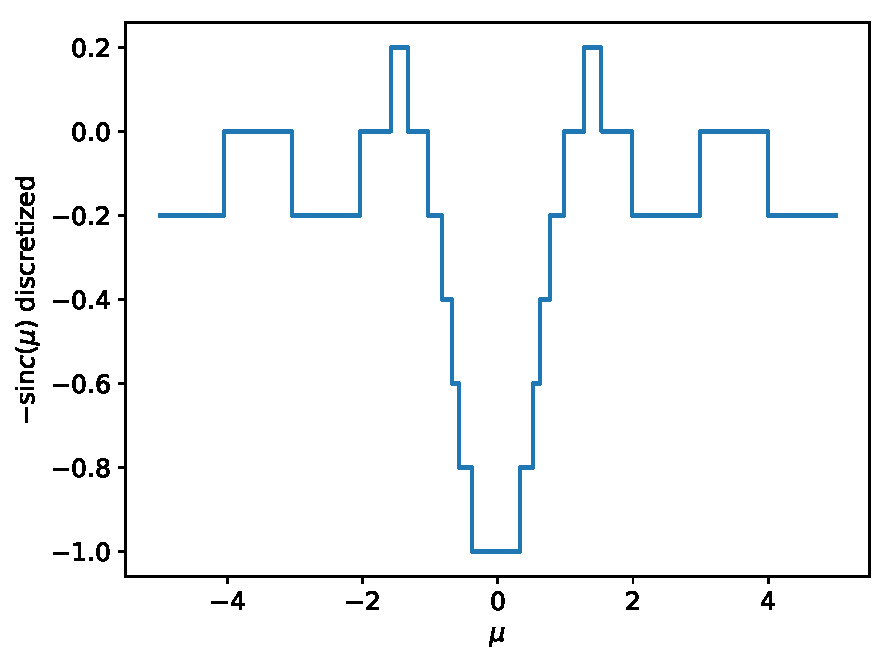
\includegraphics[width=\textwidth]{graphics/var-opt-intu/variational-optimization-function-sinc_quantized.pdf}
            \caption{}
            \label{fig: Theory: var-opt-intu-sinc-quantized-function}
        \end{subfigure}
        \hfill
        \begin{subfigure}[b]{0.49\textwidth}
            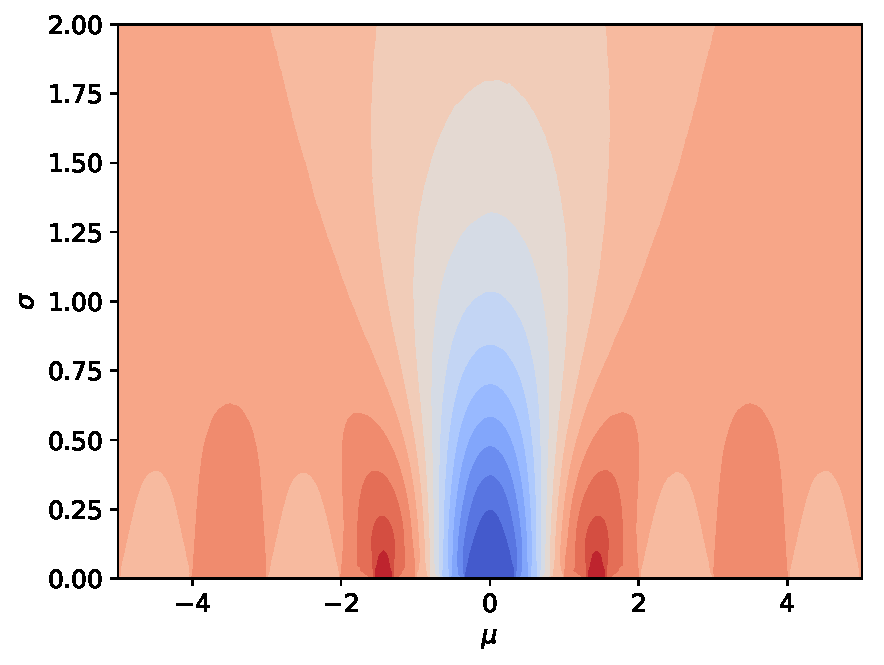
\includegraphics[width=\textwidth]{graphics/var-opt-intu/variational-optimization-contour-sinc_quantized.pdf}
            \caption{}
            \label{fig: Theory: var-opt-intu-sinc-quantized-contour}
        \end{subfigure}
        \caption{Using a univariate Gaussian search distribution, the 1-dimensional discretized and indifferentiable $\sinc$ function is turned into a 2-dimensional differentiable variational upper bound. Figures inspired by \cite{Huszar2017}.}
        \label{fig: Theory: var-opt-intu-sinc-quantized}
    \end{figure}
}


\frame{
    \begin{figure}[tbp!]
        \begin{subfigure}[b]{0.49\textwidth}
            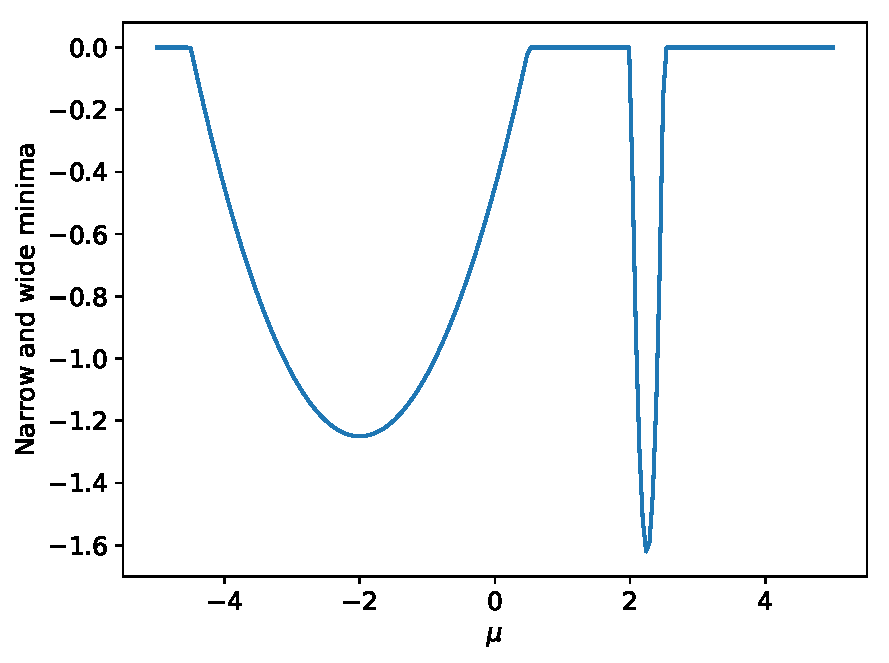
\includegraphics[width=\textwidth]{graphics/var-opt-intu/variational-optimization-function-narrow_vs_wide.pdf}
            \caption{}
            \label{fig: Theory: var-opt-intu-narrow-vs-wide-function}
        \end{subfigure}
        \hfill
        \begin{subfigure}[b]{0.49\textwidth}
            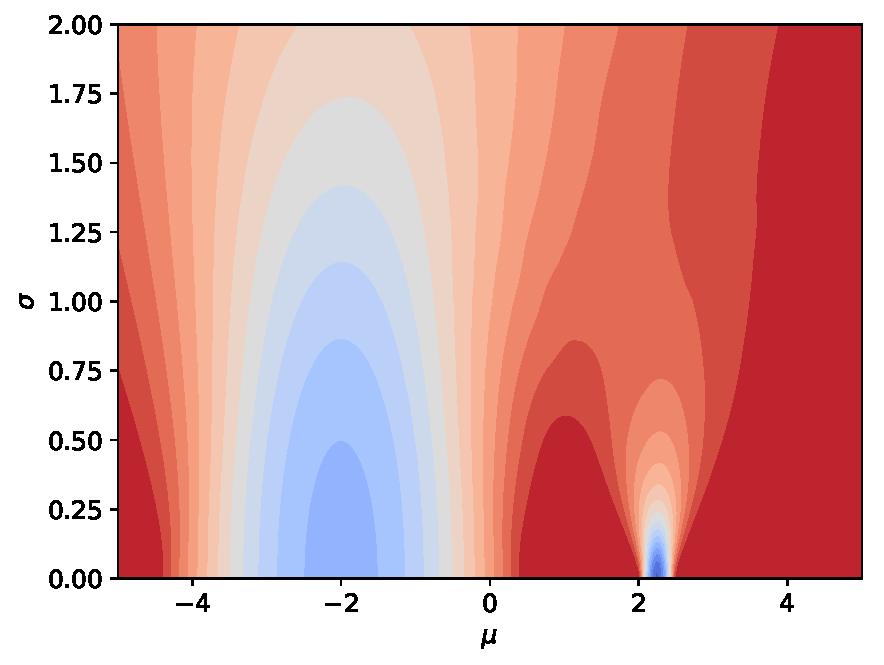
\includegraphics[width=\textwidth]{graphics/var-opt-intu/variational-optimization-contour-narrow_vs_wide.pdf}
            \caption{}
            \label{fig: Theory: var-opt-intu-narrow-vs-wide-contour}
        \end{subfigure}
        \caption{\subref{fig: Theory: var-opt-intu-narrow-vs-wide-function} A function with a low curvature local minimum and a high curvature global minimum. \subref{fig: Theory: var-opt-intu-narrow-vs-wide-contour} The contours of the corresponding Gaussian \gls{VO} objective. The Gaussian \gls{VO} objective has a different global minimum than the original function for almost all values of $\sigma>0$. This illustrates the tendency of \gls{VO} to prefer low curvature minima over high curvature minima if situated near each other. Figures inspired by \cite{Huszar2017}.}
        \label{fig: Theory: var-opt-intu-narrow-vs-wide}
    \end{figure}
}


\subsection{Natural gradient}


\frame{
    \frametitle{Natural gradient}
    \begin{block}{Problems with regular search gradients}
        \tabitem \textbf{Cannot precisely locate any optimum} since gradient explodes for $\sigma\rightarrow0$.\\
        \tabitem Want to make small change to network parameters
        \begin{equation}
            p(\w|\thetab) \leftarrow p(\w|\thetab+\Delta\thetab)
        \end{equation}
        but regular gradient defines closeness in Euclidean coordinates, $\sqrt{\Delta\thetab\transpose\Delta\thetab}$, which is dependent on search distribution parameterization and inappropriate in high dimensions.\\
        \tabitem Is it possible to obtain a gradient that is invariant to parameterization, i.e. \textbf{do gradient descent with respect to an invariant measure of the closeness of the current distribution and the updated distribution}?
    \end{block}
}


\frame{
    \frametitle{Natural gradient}
    \begin{block}{\gls{KL}}
        \tabitem Measures distance between \glspl{PDF} and is invariant to parameterization \cite{Kullback1951}.\\
        \begin{equation}
            \begin{aligned}
                \text{KL}\pa{p||q} &\equiv -\int p(\w)\log q(\w) \text{d}\w + \int p(\w)\log p(\w) \text{d}\w\\
                &= -\int p(\w)\log\pa{\frac{q(\w)}{p(\w)}}\text{d}\w
            \end{aligned}
        \end{equation}
        \tabitem It can be approximated by Taylor series
        \begin{equation}
            \text{KL}\pa{p(\w|\thetab)|| p(\w|\thetab+\Delta\thetab)} \approx \frac{1}{2}\Delta\thetab\transpose\F_\thetab\Delta\thetab
        \end{equation}
    \end{block}
    \begin{block}{Fisher information}
        \begin{align}
            \F_\thetab &\equiv \text{E}\bra{\nabla_\thetab\log p(\w|\thetab)\nabla_\thetab\log p(\w|\thetab)\transpose}\\
            &= \text{Cov}\bra{\nabla_\thetab\log p(\w|\thetab)}\\
            &= -\text{E}\bra{\nabla_\thetab^2\log p(\w|\thetab)}
        \end{align}
    \end{block}
}


\frame{
    \frametitle{Natural gradient}
    \begin{block}{Fixing the per iteration search distribution change}
        \tabitem Each minimization step on the variational upper bound can be written by a Taylor approximation as
        \begin{equation}
            U(\thetab + \Delta\thetab) \approx U(\thetab) + \Delta\thetab\transpose\nabla_\thetab U(\thetab)
        \end{equation}
        \tabitem The search gradient can then be found by minimizing the variational upper bound while keeping the \gls{KL} fixed to a small constant, $\kappa$.
        \begin{equation}
            \begin{aligned}
                &\min_\thetab U(\thetab + \Delta\thetab) \approx U(\thetab) + \Delta\thetab\transpose\nabla_\thetab U(\thetab)\\
                & \text{s.t. } \text{KL}\pa{p(\w|\thetab)|| p(\w|\thetab+\Delta\thetab)} \approx \frac{1}{2}\Delta\thetab\transpose\F_\thetab\Delta\thetab = \kappa
            \end{aligned}
        \end{equation}
        \tabitem This has the so-called natural gradient as solution
        \begin{equation}
            \tilde{\nabla}_\thetab U(\thetab) = \alpha\F_\thetab^{-1}\nabla_\thetab U(\thetab)
        \end{equation}
    \end{block}
}


\frame{
    \begin{block}{Natural gradient for univariate Gaussian}
        \tabitem Fischer information matrix can be found analytically
        \begin{equation}
            \F_\thetab = \bmat{\frac{1}{\sigma^2} & 0\\
                                0 & \frac{1}{2\sigma^4}}\quad\Longleftrightarrow\quad 
            \F_\thetab^{-1} = \bmat{\sigma^2 & 0\\
                                0 & 2\sigma^4}
        \end{equation}
        \tabitem The gradient is scaled by $\F_\thetab^{-1}$ which is analytical for the Gaussian.
        \begin{equation}
            \begin{aligned}
                \pderiv{}{\mu}U(\mu,\sigma^2) &= \sigma\text{E}\bra{f(\mu + \sigma\epsilon)\epsilon} \approx \frac{\sigma}{N}\sum_{n=1}^N f(\mu+\sigma\epsilon_n)\epsilon_n\\
                \pderiv{}{\sigma^2}U(\mu,\sigma^2) &= \sigma^2\text{E}\bra{f(\mu + \sigma\epsilon)\left(\epsilon^2-1\right)} \approx \frac{2\sigma^2}{N}\sum_{n=1}^N f(\mu + \sigma\epsilon_n)\left(\epsilon_n^2-1\right)\\
            \end{aligned}\label{eq: Theory: Variational optimization univariate gaussian gradient estimators natural gradient}
        \end{equation}
        \tabitem This can be done similarly for the isotropic and separable Gaussians.
    \end{block}
}


\subsection{Examples with natural and regular gradient}


\frame{
    \frametitle{Natural VS regular gradient - Adapting $\sigma$}
    \begin{figure}[tbp!]
        \begin{subfigure}[b]{0.49\textwidth}
            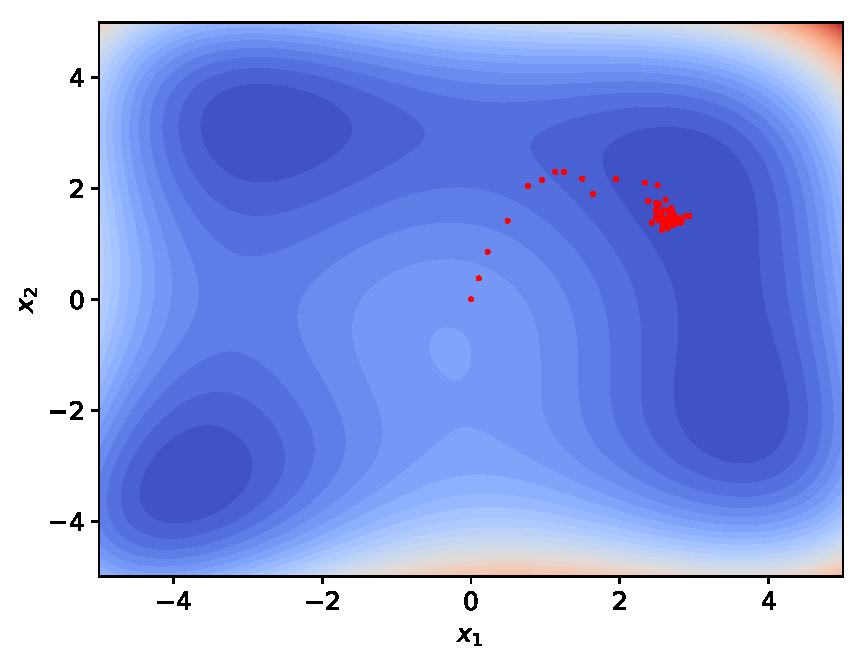
\includegraphics[width=\textwidth]{graphics/var-opt-conv/ES-himmelblau-convergence.pdf}
            \caption{}
            \label{fig: Theory: var-opt-conv-ES-himmelblau-convergence}
        \end{subfigure}
        \hfill
        \begin{subfigure}[b]{0.49\textwidth}
            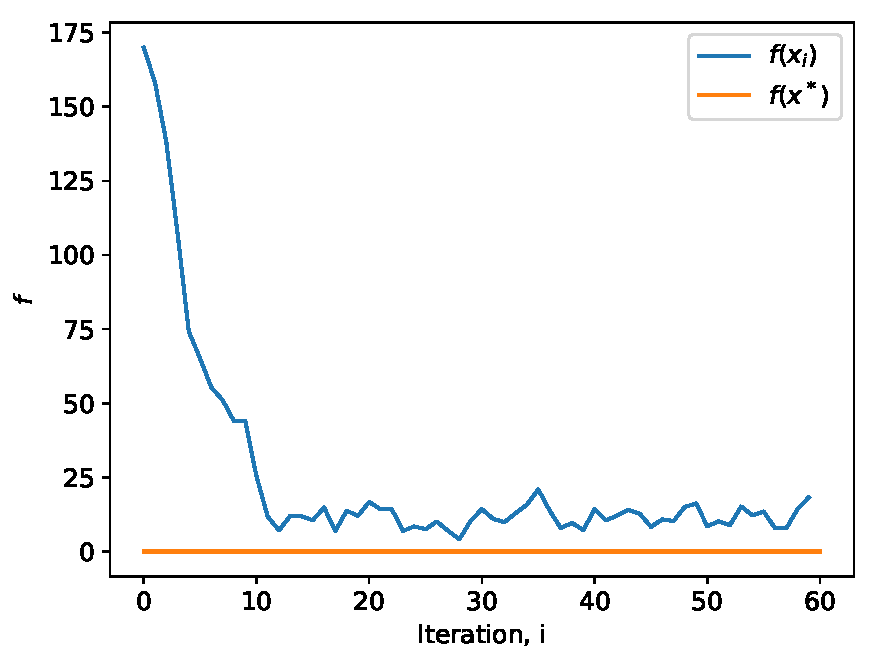
\includegraphics[width=\textwidth]{graphics/var-opt-conv/ES-himmelblau-f.pdf}
            \caption{}
            \label{fig: Theory: var-opt-conv-ES-himmelblau-f}
        \end{subfigure}
        \caption{\subref{fig: Theory: var-opt-conv-ES-himmelblau-convergence} Convergence of the "vanilla" ES algorithm with no adaptation of the variance. This is the algorithm used by \cite{Salimans2017}. \subref{fig: Theory: var-opt-conv-ES-himmelblau-f} Objective function value at each iteration of the algorithm. The algorithm finds a minimum but struggles to converge due to the fixed search distribution variance.}
        \label{fig: Theory: var-opt-conv-ES-himmelblau}
    \end{figure}
}


\frame{
    \frametitle{Natural VS regular gradient - Adapting $\sigma$}
    \begin{figure}[tbp!]
        \begin{subfigure}[b]{0.49\textwidth}
            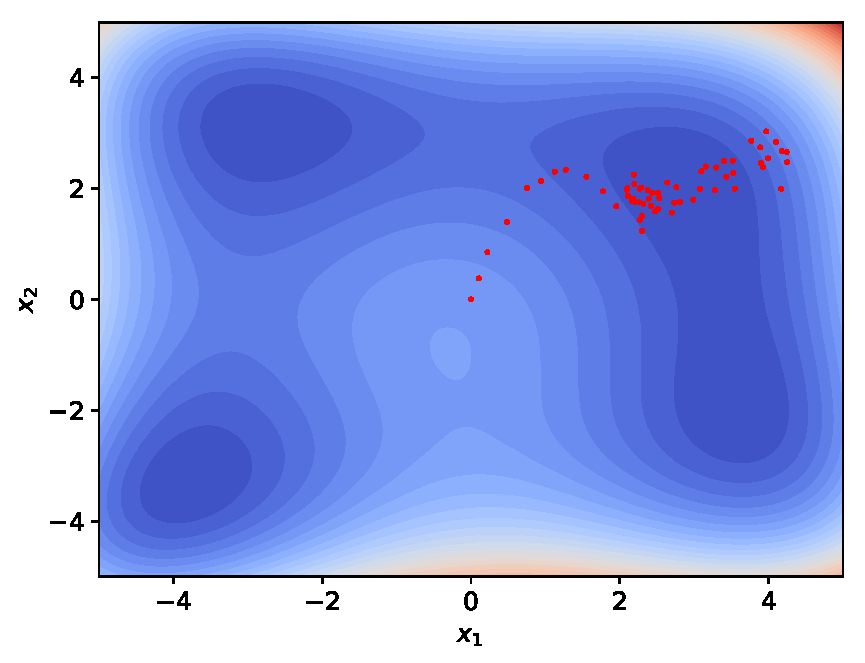
\includegraphics[width=\textwidth]{graphics/var-opt-conv/VO-R-himmelblau-convergence.pdf}
            \caption{}
            \label{fig: Theory: var-opt-conv-VO-R-himmelblau-convergence}
        \end{subfigure}
        \hfill
        \begin{subfigure}[b]{0.49\textwidth}
            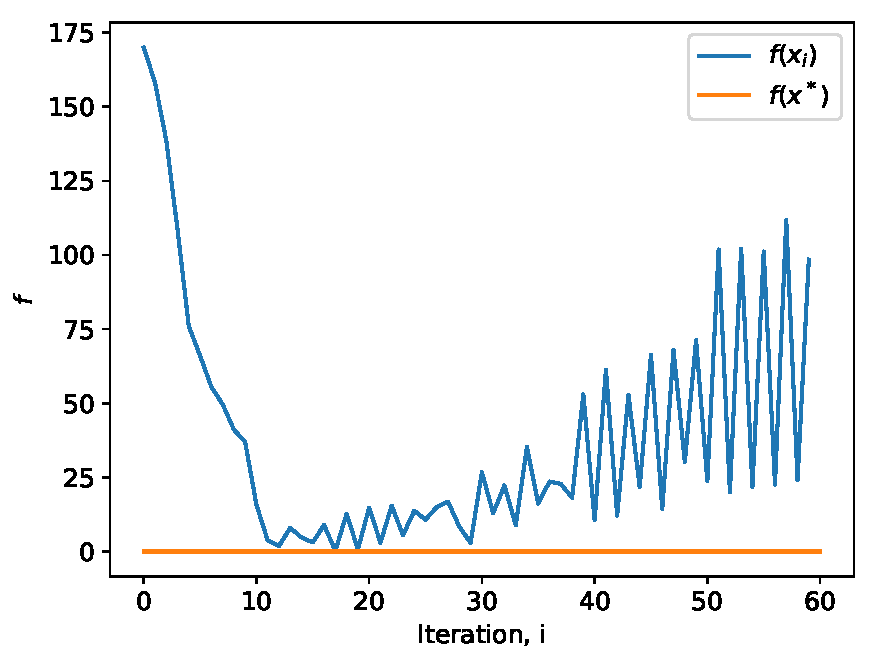
\includegraphics[width=\textwidth]{graphics/var-opt-conv/VO-R-himmelblau-f.pdf}
            \caption{}
            \label{fig: Theory: var-opt-conv-VO-R-himmelblau-f}
        \end{subfigure}
        \caption{\subref{fig: Theory: var-opt-conv-VO-R-himmelblau-convergence} Convergence of the variational optimization algorithm with isotropic Gaussian search distribution using regular gradients. \subref{fig: Theory: var-opt-conv-VO-R-himmelblau-f} Objective function value at each iteration. Similarly to "vanilla" ES, a minimum is found, but the optimization of the variance drives it towards zero, resulting in larger gradients and instability.}
        \label{fig: Theory: var-opt-conv-VO-R-himmelblau}
    \end{figure}
}


\frame{
    \frametitle{Natural VS regular gradient - Adapting $\sigma$}
    \begin{figure}[tbp!]
        \begin{subfigure}[b]{0.49\textwidth}
            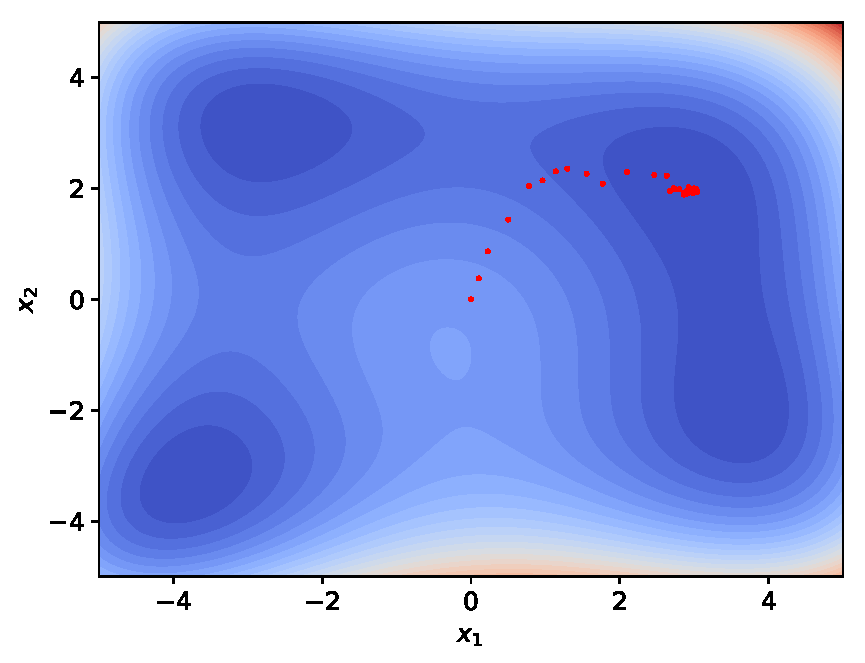
\includegraphics[width=\textwidth]{graphics/var-opt-conv/VO-N-himmelblau-convergence.pdf}
            \caption{}
            \label{fig: Theory: var-opt-conv-VO-N-himmelblau-convergence}
        \end{subfigure}
        \hfill
        \begin{subfigure}[b]{0.49\textwidth}
            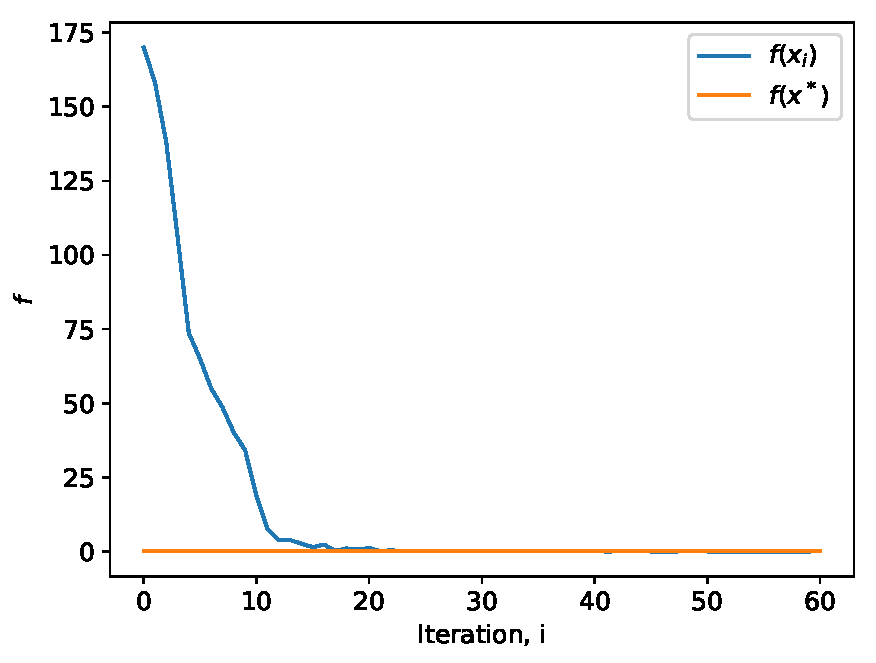
\includegraphics[width=\textwidth]{graphics/var-opt-conv/VO-N-himmelblau-f.pdf}
            \caption{}
            \label{fig: Theory: var-opt-conv-VO-N-himmelblau-f}
        \end{subfigure}
        \caption{\subref{fig: Theory: var-opt-conv-VO-N-himmelblau-convergence} Convergence of the variational optimization algorithm with isotropic Gaussian search distribution using natural gradients. \subref{fig: Theory: var-opt-conv-VO-N-himmelblau-f} Objective function value at each iteration. A minimum is found and the optimization of the variance drives the gradients toward zero resulting in convergence to the optimum.}
        \label{fig: Theory: var-opt-conv-VO-N-himmelblau}
    \end{figure}
}


\subsection{Augmentations of network and algorithm}


\frame{
    \frametitle{Augmentations}
    \begin{block}{Optimizer}
    \tabitem Any optimizer can be used.\\
    \tabitem Optimizing in $d\gg N$ regime, always moving in subspace of network weight space.\\
    \tabitem Momentum effectively works as remembering good subspace.
    \end{block}
    \begin{block}{Network architecture}
        \tabitem Batch normalization\\
        \tabitem Weight normalization\\
        \tabitem Dropout\\
        \tabitem Initialization scheme\\
    \end{block}
    \begin{block}{\gls{VO} algorithm}
    \tabitem Antithetic sampling\\
    \tabitem Safe mutations\\
    \tabitem Importance sampling\\
    \quad\tabitem Importance mixing\\
    \quad\tabitem Adaptation sampling\\
    \end{block}
}


\frame{
    \frametitle{Results for antithetic sampling}
    \begin{figure}[tbp!]
        \begin{subfigure}[b]{0.49\textwidth}
            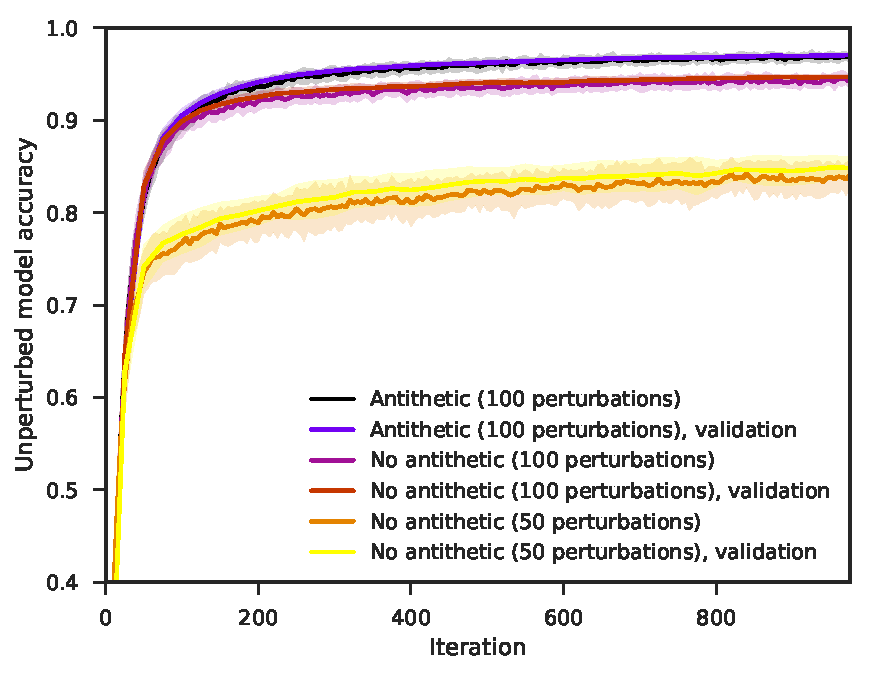
\includegraphics[width=\textwidth]{graphics/E022-AS-analysis/accuracy_unp-all-series-mean-sd.pdf}
            \caption{}
            \label{fig: Theory: E022-AS-analysis/accuracy_unp-all-series-mean-sd}
        \end{subfigure}
        \hfill
        \begin{subfigure}[b]{0.49\textwidth}
            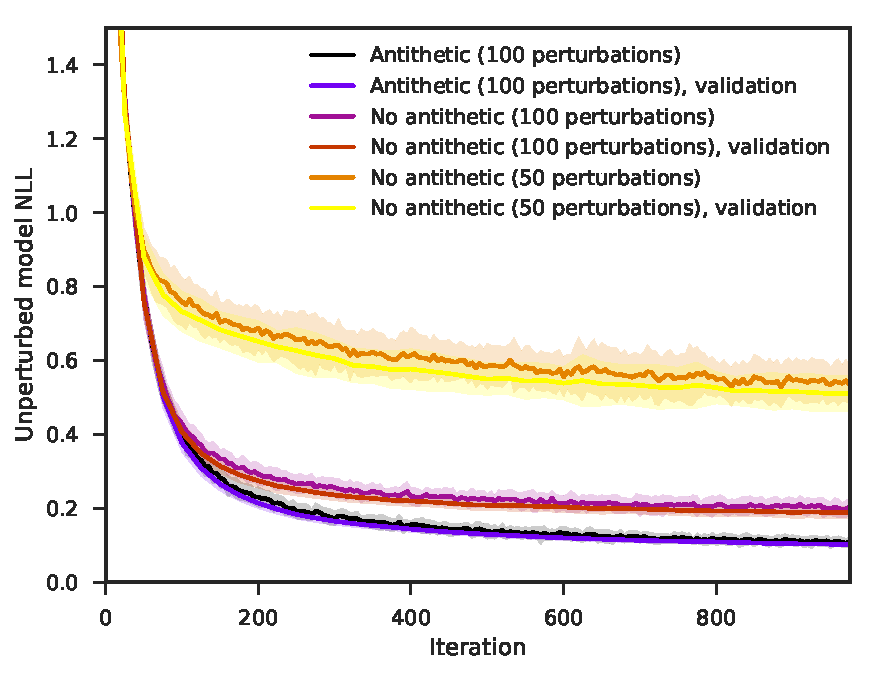
\includegraphics[width=\textwidth]{graphics/E022-AS-analysis/return_unp-all-series-mean-sd.pdf}
            \caption{}
            \label{fig: Theory: E022-AS-analysis/return_unp-all-series-mean-sd}
        \end{subfigure}
        \caption{
            Results of experiments with antithetic sampling for the unperturbed model on MNIST.
            \subref{fig: Theory: E022-AS-analysis/accuracy_unp-all-series-mean-sd} Training and validation set classification accuracy.
            \subref{fig: Theory: E022-AS-analysis/return_unp-all-series-mean-sd} Training and validation set \gls{NLL} loss.
        }
        \label{fig: Theory: E022-AS-analysis}
    \end{figure}
}


\subsection{Potential future work}


\frame{
    \frametitle{Topics for research}
    \begin{block}{Importance sampling in high dimensions}
        \tabitem How to compute importance weights in high dimensional spaces? (Importance weight collapse)\\
        \tabitem Can an alternative or approximation be made?\\
    \end{block}
    \begin{block}{Weight space VS activation space}
        \tabitem Is direct optimization in weight space necessary?\\
        \tabitem Since perturbations are normal, this provides a way to propagate perturbation distribution to activations.\\
        \tabitem One could perturb the activations and map these to weight gradients, shrinking the effective search space for fully connected linear layers \cite{Kingma2015a}.\\
    \end{block}
}

